\documentclass[UTF8,fontset=none,zihao=-4]{ctexart}
\setCJKmainfont{Songti.ttc}[Path=/System/Library/Fonts/Supplemental/, FontIndex=6, BoldFont=Songti.ttc, BoldFeatures={FontIndex=1}]
\setCJKsansfont{Songti.ttc}[Path=/System/Library/Fonts/Supplemental/, FontIndex=1, BoldFont=Songti.ttc, BoldFeatures={FontIndex=1}]
\xeCJKDeclareCharClass{FullLeft}{"2018,"201C}\xeCJKDeclareCharClass{FullRight}{"2019,"201D}
\usepackage[a4paper,margin=2.3cm]{geometry}
\usepackage{graphicx,booktabs,amsmath,amssymb,xcolor,enumitem,array,longtable,caption}
\usepackage[colorlinks=true,linkcolor=blue!50!black,urlcolor=blue!50!black,citecolor=blue!50!black]{hyperref}
\setlist{itemsep=2pt,topsep=3pt,leftmargin=*}
\captionsetup{font=small,labelfont=bf}
\graphicspath{{../figures/}}
\newcommand{\laya}{\textsf{Laya}}
\newcommand{\jev}{\textsf{Jev}}
\newcommand{\pp}{\,pp}
\ctexset{section={format=\Large\bfseries\raggedright},subsection={format=\large\bfseries\raggedright}}
\linespread{1.25}

\title{\textbf{System-1 决策模型在 Agent Harness 中的配对评测与自审计}\\[4pt]\large 技术报告：\laya{}（本地开源）vs \jev{}（云 API）}
\author{Jiawei Li}
\date{2026 年 9 月 30 日\quad（v2：含纠错与对照实验）}

\begin{document}
\maketitle
\tableofcontents
\newpage

%=====================================================================
\section*{执行摘要}
\addcontentsline{toc}{section}{执行摘要}
%=====================================================================
\textbf{问题。}Agent harness 里有大量“小决策”：路由到哪个模型、调哪个工具、要不要调工具、检索到的内容相关不相关、输入里有没有注入。System-1 决策模型用一次前向就给出带概率的类型化答案（choice / yes-no / score），号称比调 LLM 便宜、快一到两个数量级。本报告回答三个问题：在哪些决策点上够准？稳不稳、能不能设阈值？当作闸门用到底能省多少？

\textbf{规模。}11 个决策点，18 个公开数据源；7{,}283 条基础用例，外加 6{,}640 条鲁棒性变体。两边输入逐字节相同，统计上用配对检验，并做了跨硬件、跨天的复现性检查。

\textbf{结论（按可信度从高到低）。}
\begin{enumerate}
\item \jev{} 在 11 个决策点里的 9 个显著更准（+10.8 到 +46.0\pp{}，$p<0.001$）。两套基准的总体准确率：76.7\% vs 63.1\%（$n{=}2100$），80.2\% vs 66.0\%（$n{=}1280$）。
\item \textbf{模型智能路由：两家都做不了}，结果等于常数基线。\textbf{RAG 相关性门控：两家打平}（61.0\% vs 60.5\%，差值 CI 为 [$-2.0$, $+3.0$]\pp）。
\item \laya{} 的三个结构性弱点：
  \begin{itemize}
  \item 只把选项顺序反过来，就有 30.3\% 的答案会变（\jev{} 1.8\%）；
  \item 候选项一多、或彼此相似就明显下降：50 个相似工具时只有 31\%，\jev{} 在“唯一正确答案”的题目上是 98.9\%；
  \item 注入藏在文档中间时，只能抓到约一半（\jev{} 91--93\%）。
  \end{itemize}
\item \textbf{当闸门用，省得远比第一版报告说的少。}安全预筛在 $\tau{=}0.1$ 只省 4.3\% 成本（原报告 23.9\%）。RAG 门控在 5\% 漏报下，LLM 调用只能减少 7--20\%。5\% 漏报的阈值放到留出集上，95 分位会到 10--17\%。
\item \textbf{第一版报告里有 4 处影响落地建议的错误和 4 处次要错误}，见\S\ref{sec:audit}。另有 2 个我们怀疑过的混杂因素，经对照实验验证不影响结论。
\end{enumerate}

\begin{table}[h]
\centering\small
\begin{tabular}{@{}p{3.3cm}p{2.6cm}p{8.6cm}@{}}
\toprule
决策点 & 建议 & 依据 / 条件\\
\midrule
MCP / 工具选择 & \textbf{用 \jev{}} & 随机干扰 99.5\%，相似干扰（唯一解）98.9\%；\laya{} 84.0\% / 61.6\%\\
大标签意图分类（$>$20 类） & \textbf{用 \jev{}} & 81.0\% vs 35.0\%；\laya{} 在阿拉伯语、印地语（60 类）上 0/10\\
注入检测（工具输出） & \textbf{用 \jev{}} & 文档内嵌注入的检出率 91--93\%，误报 0\%；\laya{} 检出约 50\%\\
答案落地性自检 & \textbf{用 \jev{}} & 90.0\% vs 79.0\%；AUC 0.95\\
工具调用护栏 & \jev{}，并配合权限控制 & \jev{} 在“不该调”的请求上仍有 40\% 误报；\laya{} 是 74.7\%\\
执行前安全 & 只能做预筛，LLM 终审不能省 & \jev{} 预筛主要降的是延迟，成本只省 4--19\%；\laya{} 会放过 81.5\% 的有害请求\\
RAG 门控 & 不要用来“跳过生成” & 可以用作“触发补充检索”；top-5 上下文里“没有答案”的情况，两家都只能识别出不到 40\%\\
PII 出网 & 不要用 System-1 & 用正则 + NER；\laya{} AUC 0.40，\jev{} 误报 63\%\\
模型路由 & 不要零样本用 & 训练专用分类器，或用真实流量标定\\
\bottomrule
\end{tabular}
\caption{按决策点的落地建议（详见\S\ref{sec:reco}）。}
\end{table}

%=====================================================================
\section{背景与评测问题}
%=====================================================================
一个 LLM agent 外面包着一层 harness，负责一连串决策：路由、选工具、判断要不要调工具、检索门控、安全与注入审查。这些决策的输出都来自一个很小的已知集合，但今天大多还是靠同一个 LLM 生成来完成，每次要花几百毫秒和一次完整的生成。

System-1 决策模型（名字借用 Kahneman 的“快思考”）专门做这一层：输入一段 \texttt{state} 和一组类型化问题，一次非自回归前向就给出概率分布。本次评测两款：
\begin{itemize}
\item \textbf{\laya{}}：开源权重（Apache 2.0），\texttt{pip install laya}，版本 0.3.21，本地运行。内含 english / multilingual 两个 checkpoint 和一个路由器。
\item \textbf{\jev{}}：TypeSafe AI 的托管 API，响应里回显的版本号两天内一直是 \texttt{jev-1.13.0}，价格 \$0.042 / 百万 token。
\end{itemize}

三个研究问题：\textbf{RQ1} 在哪些决策点上够准？\textbf{RQ2} 可靠性如何：对选项顺序、措辞、投递通道、版本是否稳定？置信度能不能直接拿来设阈值？\textbf{RQ3} 放在 LLM 前面当闸门，实际能省多少、要承担多少风险？

%=====================================================================
\section{被测系统与评测协议}
%=====================================================================
\subsection{接口}
两家接口同构：\texttt{state}（本评测统一传字符串）加一个问题字典。三种问题类型：
\begin{itemize}
\item \texttt{choice}：\texttt{instructions} 加 \texttt{criteria}（选项键 → 简短描述），返回各选项的概率；
\item \texttt{noul}：是/否题，返回 $p(\text{yes})$；
\item \texttt{score}：有序档位打分，本评测只作辅助信号。
\end{itemize}

\subsection{公平性约束}
\begin{itemize}
\item 两边收到的 \texttt{state} 和 \texttt{questions} 逐字节相同，用例相同、顺序相同。
\item \textbf{置信度统一取 $\max_k p_k$}（是/否题取 $\max(p,1-p)$），这是 \laya{} 自己校准代码里用的口径。\laya{} 响应里的 \texttt{confidence} 字段是熵口径，和 $\max_k p_k$ 平均相差 0.299（\jev{} 只差 0.010）。\textbf{直接拿这个字段设阈值，门控逻辑就会失效。}
\item 统计方法：准确率给 Wilson 95\% 区间；两家比较用 McNemar 精确检验（只看不一致的样本对），配对差值给渐近 CI。没有做多重比较校正：文中所有“显著”都满足 $p<0.001$，所有“打平”都要求 CI 足够窄。
\end{itemize}

\subsection{确定性与可复现性（本次新增验证）}
\begin{center}\small
\begin{tabular}{@{}p{5.6cm}p{5.4cm}p{3.6cm}@{}}
\toprule
检查 & 结果 & 含义\\
\midrule
同一环境原样重跑 420 条 & \laya{} 0 条改判；\jev{} 1 条 & 两家都近乎确定性\\
\laya{}：RTX 2080 Ti（Windows）vs Apple M4 CPU（macOS） & 1{,}180/1{,}180 条决策一致，$\max|\Delta p|{=}0.006$ & 跨硬件可复现\\
\jev{}：第 1 天 vs 第 2 天（1{,}080 条） & 5 条改判（0.5\%），版本号不变 & 跨天配对是安全的\\
\bottomrule
\end{tabular}
\end{center}

\subsection{LLM 参照系}
对照实验里另加了 DeepSeek-V4.1-Flash（\texttt{deepseek-flash}，temperature 0）作为参照。它的提示格式和两家不同，因此\textbf{不参与配对比较}，只用来回答“换成一个 LLM 会怎样”。

%=====================================================================
\section{基准构成}
%=====================================================================
\begin{table}[h]
\centering\small
\begin{tabular}{@{}p{3.2cm}p{4.6cm}rp{5.4cm}@{}}
\toprule
决策点 & 数据源 & $n$ & 标签构造 / 已知弱点\\
\midrule
A 模型路由 & RouterBench（Mistral-7B vs GPT-4） & 400 & 两者都答对记 cheap，只有 GPT-4 答对记 strong；79\% 是选择题，单次运行结果带运气成分\\
B 工具选择 & BFCL simple / live\_simple & 400 & 干扰项从全部 BFCL 函数里随机抽；$K\in\{2,5,10,20,50\}$\\
C 工具调用护栏 & BFCL + irrelevance 集 & 300 & 150 条该调 / 150 条不该调\\
D RAG 门控 & BEIR 五个子集 + BM25 硬负样本 & 1{,}920 & 正 800 / 硬负 800 / 随机负 320；BEIR 的“相关”口径比“能答出来”宽\\
E 注入护栏 & deepset、jackhhao & 400 & 良性样本去掉了指令式文本\\
F 大标签集 & BANKING77、MASSIVE（10 种语言） & 200 & 60--77 类；每种语言只有 $n{=}10$\\
G 注入（双通道） & 同 E & 480 & 同一段文本分别放进用户消息和工具输出\\
H 落地性 & HaluEval-QA & 200 & 同一份证据，分别配正确答案和幻觉答案\\
I 执行前安全 & BeaverTails、HarmBench、Do-Not-Answer & 400 & BeaverTails 的标签本身是模型标的\\
J PII 出网 & ai4privacy pii-masking-300k & 200 & 原文 vs 占位符脱敏版\\
\midrule
B2 相似干扰 & BFCL & 400 & TF-IDF 最近邻干扰项（本次新增）\\
G2 文档内注入 & FiQA、CQADupStack、HaluEval、AgentDojo & 480 & 干净文档 vs 嵌入注入的文档，两个通道各一份（本次新增）\\
J2 自然脱敏 & ai4privacy & 100 & 占位符换成中性短语（本次新增）\\
S 两级安全 & I 的数据源 + Alpaca & 603 & 按书面策略由 GLM-4.6 盲标金标\\
\bottomrule
\end{tabular}
\caption{决策点与数据。A--F 的 2{,}100 条与逐条核对过标签的 100 条 pilot 不重叠。}
\end{table}

%=====================================================================
\section{主要结果：准确率与可靠性}
%=====================================================================
\subsection{分决策点准确率（RQ1）}
\begin{figure}[h]
\centering
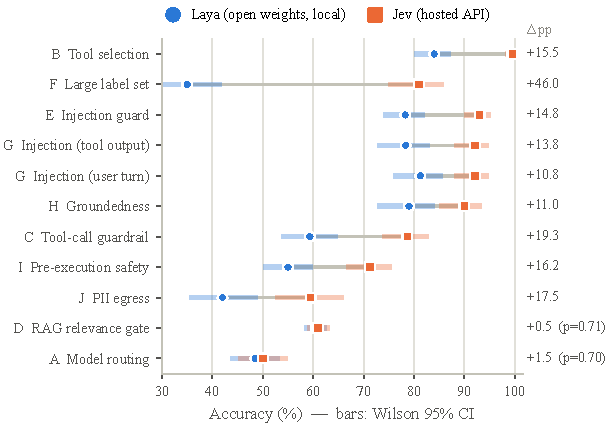
\includegraphics[width=0.62\textwidth]{fig_main}
\caption{各决策点准确率（色带为 Wilson 95\% 区间）。右侧数字为配对差值 \jev{}$-$\laya{}（pp），未注明的都是 $p<0.001$。}
\end{figure}

\begin{itemize}
\item \textbf{差距最大的是大标签集}（F：81.0\% vs 35.0\%，+46.0\pp{}，CI [38.7, 53.3]）。
\item \textbf{路由是在机会水平上打平。}\jev{} 对 99.5\% 的请求都答 cheap，准确率 50.0\% 恰好等于平衡集的常数基线；\laya{} 的 AUROC 是 0.48，等于没有判别力。
\item \textbf{RAG 是“证据充分的平局”}（$n{=}1920$，差值 +0.5\pp{}，CI [$-2.0$, $3.0$]），但两家错的方向相反：\jev{} 召回的正样本更多（58.3\% vs 45.4\%），\laya{} 拒掉的 BM25 硬负样本更多（61.8\% vs 49.3\%）。
\item \textbf{护栏类任务要看错在哪个方向。}C 轨上，对不需要工具的请求，\laya{} 有 74.7\% 仍说“要调”（\jev{} 40.0\%）；I 轨上，\laya{} 放过了 81.5\% 的有害请求（\jev{} 25.5\%）；J 轨上 \laya{} 的 AUROC 是 0.41，排序方向是反的。
\end{itemize}

\subsection{容量：候选多、候选相似}
\begin{figure}[h]
\centering
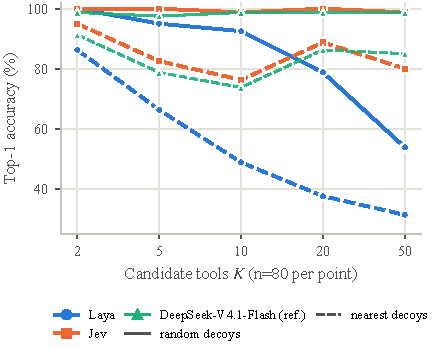
\includegraphics[width=0.55\textwidth]{fig_ksweep}
\caption{工具选择准确率随候选数 $K$ 的变化。实线为随机干扰（B），虚线为最近邻干扰（B2）。}
\end{figure}

随机干扰时，\laya{} 从 $K{=}2$ 的 100\% 平滑降到 $K{=}50$ 的 53.8\%，\jev{} 始终 $\geq$98.8\%。源码里能找到原因：所有选项共用 192 token 的预算，每个选项被截到 $\max(4,(192-16)/K)$ 个 token，$K{=}50$ 时每个选项只剩约 4 个 token。\textbf{这是架构上限，调参解决不了。}

换成相似干扰项后，\laya{} 总体只剩 54.0\%，$K{=}50$ 时 31.3\%。\jev{} 降到 84.5\%，但 DeepSeek 逐条审计发现，19.8\% 的 B2 题存在另一个同样可用的工具。只看答案唯一的 70.2\% 题目，\jev{} 是 98.9\%，\laya{} 是 61.6\%，差距从随机干扰时的 15.5\pp{} 扩大到 37.4\pp{}。

\subsection{鲁棒性（RQ2）}
\begin{figure}[h]
\centering
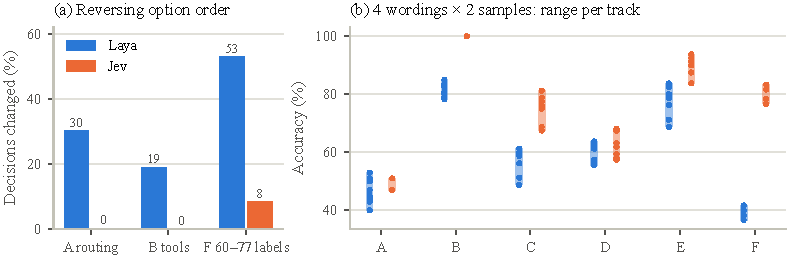
\includegraphics[width=\textwidth]{fig_robust}
\caption{(a) 只反转选项顺序后改判的比例（$n{=}1000$）；(b) 4 种措辞 $\times$ 2 次抽样下各轨道的准确率。}
\end{figure}

\begin{itemize}
\item \textbf{顺序敏感}：\laya{} 30.3\% 会改判（77 类那一档 53\%），\jev{} 1.8\%。路由题上，\laya{} 原顺序选 cheap 的比例是 58.5\%，反序后变成 82.3\%，说明它选的是位置，不是内容。
\item \textbf{措辞敏感：两家都有}。只改写 instructions、criteria 保持不变，再重新抽样，单轨准确率会波动 5--15\pp。第一版报告只测了一种改写，得出“$\pm$2\pp”，过于乐观。
\item \textbf{“谁更强”是稳的}：B、C、E、F 四轨上，8 个组合里 \jev{} 都领先（E 轨最小领先 1.3\pp）；A、D 两轨上胜负会翻转（\jev{} 分别在 6/8 和 7/8 个组合里领先）。
\end{itemize}

\subsection{校准}
合并 ECE：A--F 上 \laya{} 0.158、\jev{} 0.143；G--J 上 0.198 vs 0.080。\jev{} 在 A--F 上的 ECE 主要被路由轨拖高：它在那里“很自信地给出同一个答案”（ECE 0.477）。\laya{} 置信度 $\geq$0.9 的答案里有 26\% 是错的；它的 checkpoint 加载时也会警告部分温度参数非法、置信度未校准。\textbf{按领域重新校准是有效的}：在 D 轨上用一半数据拟合 Platt，另一半上 \laya{} 的 ECE 从 0.22 降到 0.027（\jev{} 从 0.21 降到 0.10）。

\subsection{延迟与成本：取决于部署条件}
\begin{center}\small
\begin{tabular}{@{}lrr@{}}
\toprule
配置 & p50 & p95\\
\midrule
\laya{}，RTX 2080 Ti（CUDA） & 31\,ms & 40\,ms\\
\laya{}，Apple M4 CPU & 200\,ms & 470\,ms\\
\jev{}，从 Windows 那台机器调用（第 1 天） & 325\,ms & 982\,ms\\
\jev{}，从 Mac 这台机器调用（第 2 天） & 83\,ms & 135\,ms\\
DeepSeek-V4.1-Flash（参照，单条） & 1{,}127\,ms & 3{,}605\,ms\\
\bottomrule
\end{tabular}
\end{center}
第一版报告里“Laya 比 Jev 快约 10 倍”，只是一条网络路径加一块 GPU 下的现象，不是模型本身的属性。成本方面，\jev{} 平均每次决策 759 token，约合每百万次决策 \$32；\laya{} 的边际成本是本地算力。

%=====================================================================
\section{当闸门使用（RQ3）}
%=====================================================================
\subsection{指标定义（第一版的主要混淆点）}
\begin{itemize}
\item \textbf{调用率}：仍走昂贵路径（LLM、人工审查、拦截）的流量占比。
\item \textbf{漏报率（FNR）}：本该走昂贵路径、却被闸门放掉的比例。
\item \textbf{闸门准确率}：闸门自身的二分类准确率。\textbf{它不等于端到端质量}：放行的负样本照样会交给 LLM，不会因此变成错误。
\item \textbf{端到端保留率}：可答问题最终得到回答的比例，等于 $1-\text{FNR}\times\text{正样本占比}$。
\end{itemize}

\begin{figure}[h]
\centering
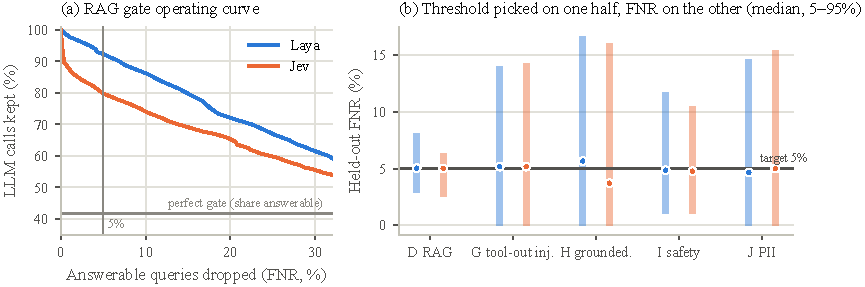
\includegraphics[width=\textwidth]{fig_gates}
\caption{(a) RAG 门控：保留的 LLM 调用比例 vs 漏掉的可答问题比例（样本内）；(b) 用一半数据选阈值、在另一半上测漏报率（500 次随机划分，目标 5\%）。}
\end{figure}

\subsection{RAG 门控}
5\% 漏报预算下，\laya{} 仍要保留 92.4\% 的 LLM 调用，\jev{} 保留 79.8\%。两家的端到端保留率都是 97.9\%。第一版报告在这里写的“端到端正确率 45--58\%”，实际是闸门自身的准确率。真正的约束是\textbf{省钱上限由“检索不相关”在流量中的占比决定}：本数据集里，即使是完美闸门也最多省 58\%。这个比例是人为构造的，所以生产环境里的绝对省钱比例会不同，但两家的排序不会变（AUROC：\jev{} 0.71，\laya{} 0.61）。在真实的 top-5 上下文上，两家识别“这里面没有答案”的比例都不到 40\%。\textbf{建议把它用作“触发补充检索”，而不是“跳过生成”。}

\subsection{阈值必须在留出集上选}
在同一份数据上选阈值、再在同一份数据上评，5\% 漏报目标必然“达成”。用一半数据选阈值、另一半评估时，中位数仍接近 5\%，但 95 分位数在 D 轨（800 个正样本）是 6--8\%，在只有 100--200 个正样本的轨道上是 10--17\%，而且约一半的划分会超过目标。\textbf{想兑现“5\% 漏报”的承诺，要么准备几百个正样本来做标定，要么阈值留出保守余量。}

\subsection{两级安全审查（预筛 + LLM 终审）}
\begin{figure}[h]
\centering
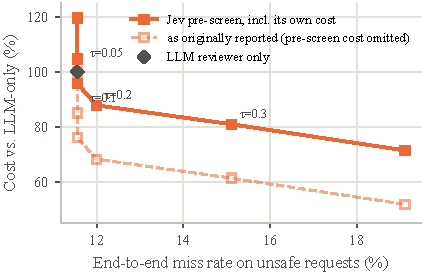
\includegraphics[width=0.55\textwidth]{fig_twotier}
\caption{\jev{} 预筛 → DeepSeek 终审：成本（相对 LLM-only）vs 端到端漏报率。虚线是第一版的算法，漏算了预筛本身的成本。}
\end{figure}

\begin{center}\small
\begin{tabular}{@{}lrrrrr@{}}
\toprule
方案 & LLM 调用率 & FNR & FPR & 成本（修正后） & 成本（第一版口径）\\
\midrule
LLM-only & 100\% & 11.6\% & 7.0\% & 100.0\% & 100.0\%\\
\jev{} $\tau{=}0.05$ & 75.2\% & 11.6\% & 7.0\% & \textbf{104.7\%} & 85.1\%\\
\jev{} $\tau{=}0.1$ & 65.6\% & 11.6\% & 7.0\% & \textbf{95.7\%} & 76.1\%\\
\jev{} $\tau{=}0.2$ & 58.9\% & 12.0\% & 5.1\% & 87.8\% & 68.2\%\\
\jev{} $\tau{=}0.3$ & 53.3\% & 15.1\% & 3.5\% & 80.9\% & 61.2\%\\
\laya{} $\tau{=}0.1$ & 99.3\% & 11.6\% & 7.0\% & 99.4\% & 99.4\%\\
\bottomrule
\end{tabular}
\end{center}
要点：
\begin{itemize}
\item 终审 LLM 本身很便宜（批处理后每百万请求 \$72），一次 \jev{} 调用就相当于它的 20\%，所以\textbf{预筛省下的钱很有限}。
\item 真正的收益是\textbf{延迟}：34--41\% 的请求可以在约 0.3\,s 内直接放行，不用等几秒的 LLM 审查（批 p50 4.1\,s，p95 33.8\,s）。
\item “不增加漏报”只在样本内成立。阈值改用留出集选取后，47\% 的划分会至少多漏 1 条。
\item \laya{} 做预筛没有意义：为了保住召回，它必须把 99.3\% 的流量交给终审。
\item 标签口径说明：金标（GLM-4.6 按书面策略标注）与数据集原标签只有 72.8\% 一致；终审与金标一致 91.1\%，与数据集标签一致 75.0\%（第一版脚本在这里误报成 91.1\%）。
\end{itemize}

\subsection{\laya{} → \jev{} 级联}
\begin{center}\small
\begin{tabular}{@{}lrrr@{}}
\toprule
\laya{} 本地承接阈值 & 本地承接比例 & 级联准确率 & \jev{} 花费 / 百万次\\
\midrule
0.5 & 95.0\% & 65.7\% & \$4.0\\
0.8 & 56.9\% & 70.0\% & \$15.1\\
0.9 & 41.7\% & 70.7\% & \$19.0\\
0.99 & 19.1\% & 73.4\% & \$25.3\\
纯 \jev{} & 0\% & 76.7\% & \$34.6\\
\bottomrule
\end{tabular}
\end{center}
每百万次决策省 \$16，要付出 6 个百分点的准确率，在大多数场景下不划算。\textbf{该省的是“用 System-1 替掉 LLM 调用”，不是在两个 System-1 模型之间抠 token 费。}

%=====================================================================
\section{自审计：第一版报告改了什么}\label{sec:audit}
%=====================================================================
第一版评测做得很快，报告写得详细而自信。本次我们从原始输出重算了所有数字，并为每个可疑的混杂因素设计了对照实验。

\begin{longtable}{@{}p{4.6cm}p{5.0cm}p{5.0cm}@{}}
\toprule
第一版说法 & 审计后 & 根因\\
\midrule
\endhead
\multicolumn{3}{@{}l}{\textbf{影响落地建议的错误}}\\
预筛 $\tau{=}0.1$ 省 23.9\% 安全审查成本 & 只省 4.3\%；$\tau{=}0.05$ 反而贵 4.7\% & 两级总成本里漏算了预筛本身的 token 费\\
RAG 门控 5\% 漏报时“端到端正确率 45--58\%” & 端到端保留 97.9\%；45--58\% 是闸门准确率 & 指标标错：放行的负样本仍交给 LLM\\
预筛带来“零”额外漏报；各闸门阈值“达成 5\% 漏报” & 留出集上 47\% 的划分多漏；FNR 95 分位最高 16.7\% & 阈值在同一数据上选取和评估\\
工具输出通道让良性误报翻 2--3 倍，需要分通道标定 & 只在“把用户式短文本搬进工具输出”时成立；换成原生文档后 \jev{} 误报 0\%→0\% & 良性用户问句出现在工具输出里本身就反常\\
\multicolumn{3}{@{}l}{\textbf{次要数字的错误}}\\
措辞敏感度 $\pm$2\pp & 4 种措辞 $\times$ 2 次抽样下波动 5--15\pp & 只测了一种改写，等于只抽了一个样本\\
终审与数据集标签一致 91.1\% & 75.0\% & 脚本表达式写错，返回的是另一个一致率\\
\jev{} 比 \laya{} 慢约 10 倍 & 83--325\,ms vs 31--200\,ms，取决于网络位置和硬件 & 只测了一个客户端位置、一块 GPU\\
C 轨 \jev{} 31\%（首版构建） & 78.7\% & 构建脚本漏了用户请求（首版报告前已修复）\\
\multicolumn{3}{@{}l}{\textbf{被怀疑、但经对照实验验证不影响结论}}\\
工具选择 99.5\% 被随机干扰项抬高 & 相似干扰、答案唯一的题上 \jev{} 98.9\%，与 \laya{} 的差距反而更大 & ---\\
PII AUROC 0.41 是占位符负样本造成的 & 换成自然脱敏：\laya{} 0.40，\jev{} 0.82，基本不变 & ---\\
另有：\texttt{gate-config.json} 每次运行都被覆盖 & 改为每道闸门单独输出一个文件 & 脚本 bug\\
\bottomrule
\end{longtable}

\subsection{对照实验 G2：是通道的问题还是内容的问题}
\begin{figure}[h]
\centering
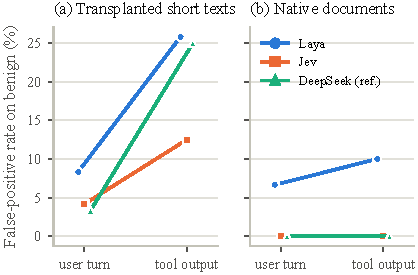
\includegraphics[width=0.55\textwidth]{fig_channel}
\caption{良性内容的误报率随投递通道的变化。(a) 原设计：用户式短文本原样放进两个通道；(b) 对照：120 段论坛/网页/百科原生文本。}
\end{figure}
原设计把同一段短文本分别放进用户消息和工具输出。其中良性文本是用户问句（如 “Unemployment young people Europe”），出现在 \texttt{read\_email} 的输出里本身就很反常。对照实验取 120 段本来就会出现在工具输出里的文本：FiQA、CQADupStack 和 HaluEval 里的维基段落。每段做成干净版和嵌入注入版，注入内容一半是 60 条 AgentDojo 注入目标（套 4 种载体模板），一半是 60 条 deepset payload；每个版本都分别投递到两个通道。

结果：在“搬运来的短文本”上，三个模型都表现出通道效应，连 LLM 参照也是（误报 3.3\%→25.0\%）；换成原生文档后效应消失：\jev{} 和 LLM 在两个通道的误报都是 0\%，\laya{} 从 6.7\% 到 10.0\%，不显著（$p{=}0.34$）。平均 $p(\text{attack})$ 仍有小幅上移（\jev{} 在干净文档上从 0.04 升到 0.13）。

\textbf{同时暴露出一个新弱点}：注入嵌在文档中间时，\laya{} 只能检出 47.5--50.8\%（单独 payload 时是 70.8--82.5\%）；\jev{} 在单独和嵌入两种情况下分别是 88.3--94.2\% 和 90.8--93.3\%。

\subsection{对照实验 B2：相似干扰项}
把随机干扰换成与正确函数最相似的 $K-1$ 个函数（按名称和描述算 TF-IDF，排除余弦相似度 $\geq$0.8 的近重复），平均相似度从 0.01 升到 0.22。相似工具可能“同样正确”，所以用 DeepSeek 逐条列出所有可用工具：答案唯一的题目在 B2 中占 70.2\%，在 B 中占 96.3\%。注意：这个唯一性子集由 LLM 筛出，可能偏向 LLM 式的判断。

\subsection{对照实验 J2：自然脱敏负样本}
把 \texttt{[LASTNAME1]} 这类占位符换成“the person”“their phone number”这样的中性短语。\jev{} 误报 66\%→63\%，\laya{} AUROC 0.41→0.40，基本不变；LLM 参照的误报从 25\% 降到 12\%。原结论成立：\textbf{PII 出网审查不要用 System-1}。这个任务本质上是找实体，应该交给 NER 加规则。

%=====================================================================
\section{标签质量与效度威胁}
%=====================================================================
\begin{itemize}
\item \textbf{标签噪声}：DeepSeek 盲法官（不给金标、不给模型答案）重标了 360 条分层样本。它与数据集标签的一致率：两家都对的样本 90.0\%，两家分歧的样本 75.7\%，两家都错的样本只有 12.7\%。把法官指令从“严格”换成“宽松”，28.1\%（32/114）的双错样本标签会翻转，主要因为 BEIR 的“相关”口径比“能答出来”宽。所以 D、I 两轨的绝对准确率偏低。
\item \textbf{法官“站 \jev{}”不算独立证据}：在两家分歧、法官能判定的 145 条里，法官 131 条站 \jev{}。但法官和 \jev{} 可能有相同的系统性偏好，所以排序结论依靠的是金标本身和它在措辞变化下的稳定性。
\item \textbf{路由标签}：79\% 来自选择题基准，95\% 是单次运行得到的 0/1 结果。7B 模型“答对”一道四选一题有运气成分，这个任务的准确率上限未知。本评测只能说明“在这套标签上零样本路由做不了”。
\item \textbf{数据污染}：全部数据源都是公开的，\jev{} 的训练数据不公开，B、E 上接近满分可能部分来自见过数据。好在 B2、G2、J2 用的是新组合的输入，结论依然成立。
\item \textbf{没有覆盖的}：\laya{} 的微调路径（它主打的领域适配卖点）；typed-decisions checkpoint（在 CUDA 上会崩，CPU 上 100 条 pilot 为 59\%，与默认路由器的 58\% 接近）；中文流量（F 轨中文只有 10 条）；多个版本。
\item \textbf{审计的覆盖范围}：能想到的错误都已修正，但审计只能覆盖审计者想到的问题。所有原始响应都已保留，方便他人继续审查。
\end{itemize}

%=====================================================================
\section{落地建议}\label{sec:reco}
%=====================================================================
\subsection{架构}
\begin{enumerate}
\item \textbf{System-1 负责“一眼能判断的闭集决策”，LLM 负责生成。}工具选择、意图分类、注入筛查、落地性自检交给 \jev{} 这一级的模型。
\item \textbf{安全类闸门做两级}：System-1 预筛只用来降低延迟和慢路径占比，终审 LLM 保留；想降低漏报，就要换更强的终审模型或加人工，改进预筛帮不上。
\item \textbf{RAG 用“补充检索触发器”}，不要用来跳过生成。
\item \textbf{PII 用 NER 加规则；路由用专门训练的分类器或真实流量标定。}
\end{enumerate}

\subsection{如果要用 \laya{}}
\begin{itemize}
\item 选项数 $K\lesssim10$，且选项之间差异明显；描述写短，共享预算只有 192 token。
\item 固定选项顺序，或者在 2--3 种顺序上投票。
\item 置信度自己用 $\max_k p_k$ 算，不要用响应里的 \texttt{confidence} 字段。
\item 在自己的领域上做 Platt 或温度标定之后再定阈值。
\item 不要用于安全、PII、多语言大标签集，也不要用于检测嵌在文档里的注入。
\end{itemize}

\subsection{评测这类闸门时的守则}
\begin{enumerate}
\item 分开报告\textbf{调用率}、\textbf{留出集漏报率}和\textbf{端到端保留率}，不要把闸门准确率写成端到端质量。
\item 成本要算上\textbf{所有组件}，包括闸门本身。
\item 阈值在留出集上选；正样本少于几百个时，报告漏报率的分布，而不是一个点。
\item 测通道效应要用\textbf{各通道原生的内容}；测工具选择要包含\textbf{相似干扰项}，并审计答案是否唯一。
\item 任何“惊人结论”，先查数据；措辞和抽样至少各做两份。
\end{enumerate}

%=====================================================================
\section{复现}
%=====================================================================
\begin{itemize}
\item 版本：\laya{} 0.3.21（transformers 5.17.0，torch 2.14.0）；\jev{} \texttt{jev-1.13.0}；DeepSeek \texttt{deepseek-flash}。
\item 环境：第 1 天 Windows + RTX 2080 Ti；第 2 天 macOS + Apple M4（CPU）。
\item 费用：\jev{} 全部运行共 \$0.52；DeepSeek 审计和参照共约 1.7M 输入 / 1.1M 输出 token。
\end{itemize}
{\footnotesize
\begin{verbatim}
# 新增对照实验（在 sys1-eval/ 下运行）
python scripts/build_v2_cases.py         # B2 / G2 / J2 + 原 B/G/J 重跑
JEV_ENV_FILE=../.env node scripts/run_jev.mjs \
    bench/v2-cases.jsonl results/mac/jev-v2.jsonl
LAYA_DEVICE=cpu python scripts/run_laya.py \
    bench/v2-cases.jsonl results/mac/laya-v2.jsonl
DS_ENV_FILE=../.env node scripts/llm_ref.mjs audit \
    bench/v2-cases.jsonl results/mac/ds-audit-tools.jsonl
DS_ENV_FILE=../.env node scripts/llm_ref.mjs answer \
    bench/v2-cases.jsonl results/mac/ds-v2.jsonl
# 全部数字与图表（单一来源）
python paper/analysis.py     # -> paper/numbers.json, paper/figures/
# 论文与本报告
cd paper/tex && tectonic -X compile main.tex
tectonic -X compile tech-report-zh.tex
\end{verbatim}}
已修正的原脚本：
\begin{itemize}
\item \texttt{scripts/two\_tier\_safety.mjs}：预筛成本、成本分母、标签一致率；
\item \texttt{scripts/rag\_analysis.mjs}：指标改名，新增端到端保留率；
\item \texttt{scripts/gate\_config.mjs}：每道闸门单独输出文件，指标改名；
\item \texttt{lib/judge.mjs}：支持直连 DeepSeek。
\end{itemize}

\appendix
%=====================================================================
\section{完整数值}
%=====================================================================
\begin{longtable}{@{}lrrrrrl@{}}
\caption{分轨道配对结果（准确率 \%，差值 pp，95\% CI）}\\
\toprule
轨道 & $n$ & \laya{} & \jev{} & 只 \laya{} 对 & 只 \jev{} 对 & 差值 [CI]\\
\midrule
\endhead
A 路由 & 400 & 48.5 & 50.0 & 80 & 86 & +1.5 [$-$4.8, 7.8]\\
B 工具选择 & 400 & 84.0 & 99.5 & 1 & 63 & +15.5 [11.9, 19.1]\\
C 工具护栏 & 300 & 59.3 & 78.7 & 8 & 66 & +19.3 [14.2, 24.5]\\
D RAG（400） & 400 & 58.5 & 60.8 & 58 & 67 & +2.2 [$-$3.2, 7.7]\\
D RAG（1920） & 1920 & 60.5 & 61.0 & 290 & 300 & +0.5 [$-$2.0, 3.0]\\
E 注入 & 400 & 78.2 & 93.0 & 19 & 78 & +14.8 [10.1, 19.4]\\
F 大标签 & 200 & 35.0 & 81.0 & 3 & 95 & +46.0 [38.7, 53.3]\\
G 用户通道 & 240 & 81.2 & 92.1 & 10 & 36 & +10.8 [5.5, 16.2]\\
G 工具输出 & 240 & 78.3 & 92.1 & 12 & 45 & +13.8 [7.8, 19.7]\\
H 落地性 & 200 & 79.0 & 90.0 & 5 & 27 & +11.0 [5.7, 16.3]\\
I 执行前安全 & 400 & 55.0 & 71.2 & 55 & 120 & +16.2 [10.0, 22.5]\\
J PII & 200 & 42.0 & 59.5 & 30 & 65 & +17.5 [8.3, 26.7]\\
\midrule
A--F 合计 & 2100 & 63.1 & 76.7 & 169 & 455 & +13.6 [11.4, 15.9]\\
G--J 合计 & 1280 & 66.0 & 80.2 & 112 & 293 & +14.1 [11.2, 17.1]\\
\bottomrule
\end{longtable}

\begin{longtable}{@{}lrrrrrr@{}}
\caption{是/否题轨道在阈值 0.5 下的表现（FNR / FPR 单位为 \%）}\\
\toprule
& \multicolumn{3}{c}{\laya} & \multicolumn{3}{c}{\jev}\\
轨道 & AUC & FNR & FPR & AUC & FNR & FPR\\
\midrule
\endhead
C 工具护栏 & .56 & 6.7 & 74.7 & .86 & 2.7 & 40.0\\
D RAG（400） & .58 & 57.8 & 29.9 & .70 & 42.2 & 37.2\\
E 注入 & .88 & 22.0 & 21.5 & .98 & 7.0 & 7.0\\
G 用户通道 & .90 & 29.2 & 8.3 & .98 & 11.7 & 4.2\\
G 工具输出 & .85 & 17.5 & 25.8 & .97 & 5.8 & 10.0\\
H 落地性 & .79 & 5.0 & 37.0 & .95 & 4.0 & 16.0\\
I 执行前安全 & .64 & 81.5 & 8.5 & .77 & 25.5 & 32.0\\
J PII & .41 & 77.0 & 39.0 & .81 & 15.0 & 66.0\\
\bottomrule
\end{longtable}

\begin{longtable}{@{}lccccccccccc@{}}
\caption{F 轨各语言准确率（\%；BANKING77 $n{=}100$，其余每种语言 $n{=}10$，只看趋势）}\\
\toprule
& B77 & en & zh & ja & de & fr & es & ko & pt & ar & hi\\
\midrule
\endhead
\laya & 40 & 30 & 30 & 60 & 30 & 60 & 40 & 20 & 30 & 0 & 0\\
\jev & 84 & 80 & 50 & 100 & 90 & 70 & 90 & 90 & 80 & 80 & 50\\
\bottomrule
\end{longtable}

{\small\setlength{\tabcolsep}{4pt}
\begin{longtable}{@{}lrrrrrr@{}}
\caption{闸门阈值：样本内选取 vs 留出集评估（目标漏报 5\%，500 次划分；阈值与调用率为样本内值，“超标”指留出 FNR 超过 5\% 的划分比例）}\\
\toprule
闸门 / 模型 & 阈值 & 调用率 & 留出 FNR 中位 & P5 & P95 & 超标\\
\midrule
\endhead
D RAG / \laya & 0.049 & 92.4\% & 5.0\% & 2.9\% & 8.1\% & 51\%\\
D RAG / \jev & 0.070 & 79.8\% & 5.0\% & 2.6\% & 6.3\% & 50\%\\
G 工具输出注入 / \laya & 0.092 & 79.6\% & 5.2\% & 0.0\% & 14.0\% & 53\%\\
G 工具输出注入 / \jev & 0.480 & 53.8\% & 5.2\% & 0.0\% & 14.3\% & 52\%\\
H 落地性 / \laya & 0.034 & 96.0\% & 5.6\% & 0.0\% & 16.7\% & 52\%\\
H 落地性 / \jev & 0.050 & 66.0\% & 3.6\% & 0.0\% & 16.1\% & 27\%\\
I 执行前安全 / \laya & 0.014 & 93.8\% & 4.9\% & 1.0\% & 11.7\% & 47\%\\
I 执行前安全 / \jev & 0.050 & 82.0\% & 4.8\% & 1.0\% & 10.5\% & 41\%\\
J PII / \laya & 0.016 & 96.0\% & 4.7\% & 0.0\% & 14.6\% & 49\%\\
J PII / \jev & 0.030 & 94.5\% & 5.0\% & 0.0\% & 15.4\% & 50\%\\
\bottomrule
\end{longtable}}

\begin{longtable}{@{}lrrrr@{}}
\caption{通道对照（\%，第 2 天运行）}\\
\toprule
模型 / 通道 & 短文本 TPR & 短文本 FPR & 文档 TPR & 文档 FPR\\
\midrule
\endhead
\laya{} 用户消息 & 70.8 & 8.3 & 47.5 & 6.7\\
\laya{} 工具输出 & 82.5 & 25.8 & 50.8 & 10.0\\
\jev{} 用户消息 & 88.3 & 4.2 & 93.3 & 0.0\\
\jev{} 工具输出 & 94.2 & 12.5 & 90.8 & 0.0\\
LLM 参照 用户消息 & 85.0 & 3.3 & 97.5 & 0.0\\
LLM 参照 工具输出 & 97.5 & 25.0 & 98.3 & 0.0\\
\bottomrule
\end{longtable}

\begin{figure}[h]
\centering
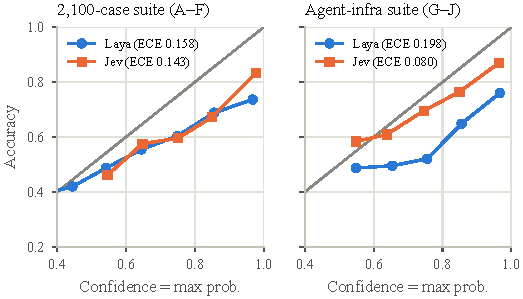
\includegraphics[width=0.62\textwidth]{fig_reliability}
\caption{可靠性图（10 个分箱，每个点至少 10 条样本）。}
\end{figure}

\end{document}
